\documentclass{segabs}
\usepackage{xspace,color,amsmath}
\usepackage{amssymb}
\usepackage{hyperref}

\begin{document}

\title{Machine learning for the classification of unexploded ordnance (UXO) from electromagnetic data}

\author{
    Lindsey J. Heagy$^1$, Douglas W. Oldenburg$^2$, Fernando P\'erez$^1$ \& Laurens Beran$^3$ \\
    $^1$Department of Statistics, University of California Berkeley \\
    $^2$Geophysical Inversion Facility, University of British Columbia \\
    $^3$Black Tusk Geophysics
}
\email{lheagy@berkeley.edu}

% \footer{Example}
% \lefthead{Heagy, Oldenburg, P\'erez \& Beran}
% \righthead{Machine learning for the classification of UXO}

\maketitle

\begin{abstract}
% \vspace{-0.6cm}

Electromagnetic methods are widely used for the detection and classification of unexploded ordnance objects in former war zones or military training grounds. Typically, targets are classified using intrinsic parameters that are estimated via inversion of the observed data. In this work, we present an approach for using convolutional neural networks to classify unexploded ordnance directly from time-domain electromagnetic data. The outputs of the network are probabilities that the signal in a given spatial window is associated with an ordnance object, as well as a classification, which is simply the class with the largest probability. We demonstrate our approach with a synthetic example and show that the trained neural network can distinguish between small, medium, and large ordnance objects, as well as metallic clutter, and background response. These results illustrate the potential utility of machine learning for the interpretation of electromagnetic data collected over sites contaminated with ordnance.

\end{abstract}

% \vspace{-0.45cm}
\section{Introduction and motivation}
% \vspace{-0.25cm}

Unexploded ordnance (UXO) are munitions that were armed, fired and remain unexploded. They are a hazard in countries that have had active wars or military training grounds. In the US alone, it is estimated that there are on the order of 10 million acres of land at over 1400 sites that are contaminated with UXO; the associated clean-up costs are in the 10s of billions \citep{Etter2003}. Improving classification to better identify items  which must be dug up, and distinguish them from clutter, which may safely be left in the ground, can significantly reduce these costs.

UXO items have a significant magnetic permeability and are electrically conductive, so they may be detected with magnetic or electromagnetic techniques. For the classification step, we require data that have sufficient information-content to allow us to extract features or estimate parameters that can be used to distinguish between ordnance items and clutter. Multi-component time-domain electromagnetic (TDEM) systems have proven to be well-suited for this task (cf. \cite{Bell2001, Pasion2001, Zhang2003, Billings2010}).

To interpret the TDEM data and associate an observed signal with an ordnance item, a common approach is to conduct a series of inversions to estimate the location, orientation, and electromagnetic properties of the target and then match these properties to a library of known ordnance objects \cite{Andrews2011, Beran2013}. These parametric inversions are non-linear and prone to getting stuck in local minima. Given the success of neural networks for classification tasks, not only for images, but also for scientific data, the question we pose is: can we construct a neural network to classify ordnance objects directly from TDEM data without performing an inversion? Specifically of interest is to obtain the probability that an observed signal is associated with a given ordnance object.

% \vspace{-0.45cm}
\section{Modelling the electromagnetic response of a UXO}
% \vspace{-0.25cm}

Figure \ref{fig:uxo-coordinates} demonstrates the setup of a time-domain electromagnetic experiment to detect and classify an ordnance object. A transmitter generates a time-varying magnetic field $\mathbf{h}_T$ which induces eddy currents in the conductive, permeable ordnance object. These eddy currents produce a secondary magnetic field $\mathbf{h}_R$. At the receiver location, we measure the time-rate-of-change of the secondary magnetic flux ($\partial \mathbf{b}_R/\partial t = \mu_0 \partial \mathbf{h}_R/\partial t$).

\begin{figure}[htb]
% \vspace{-0.1cm}
    \begin{center}
    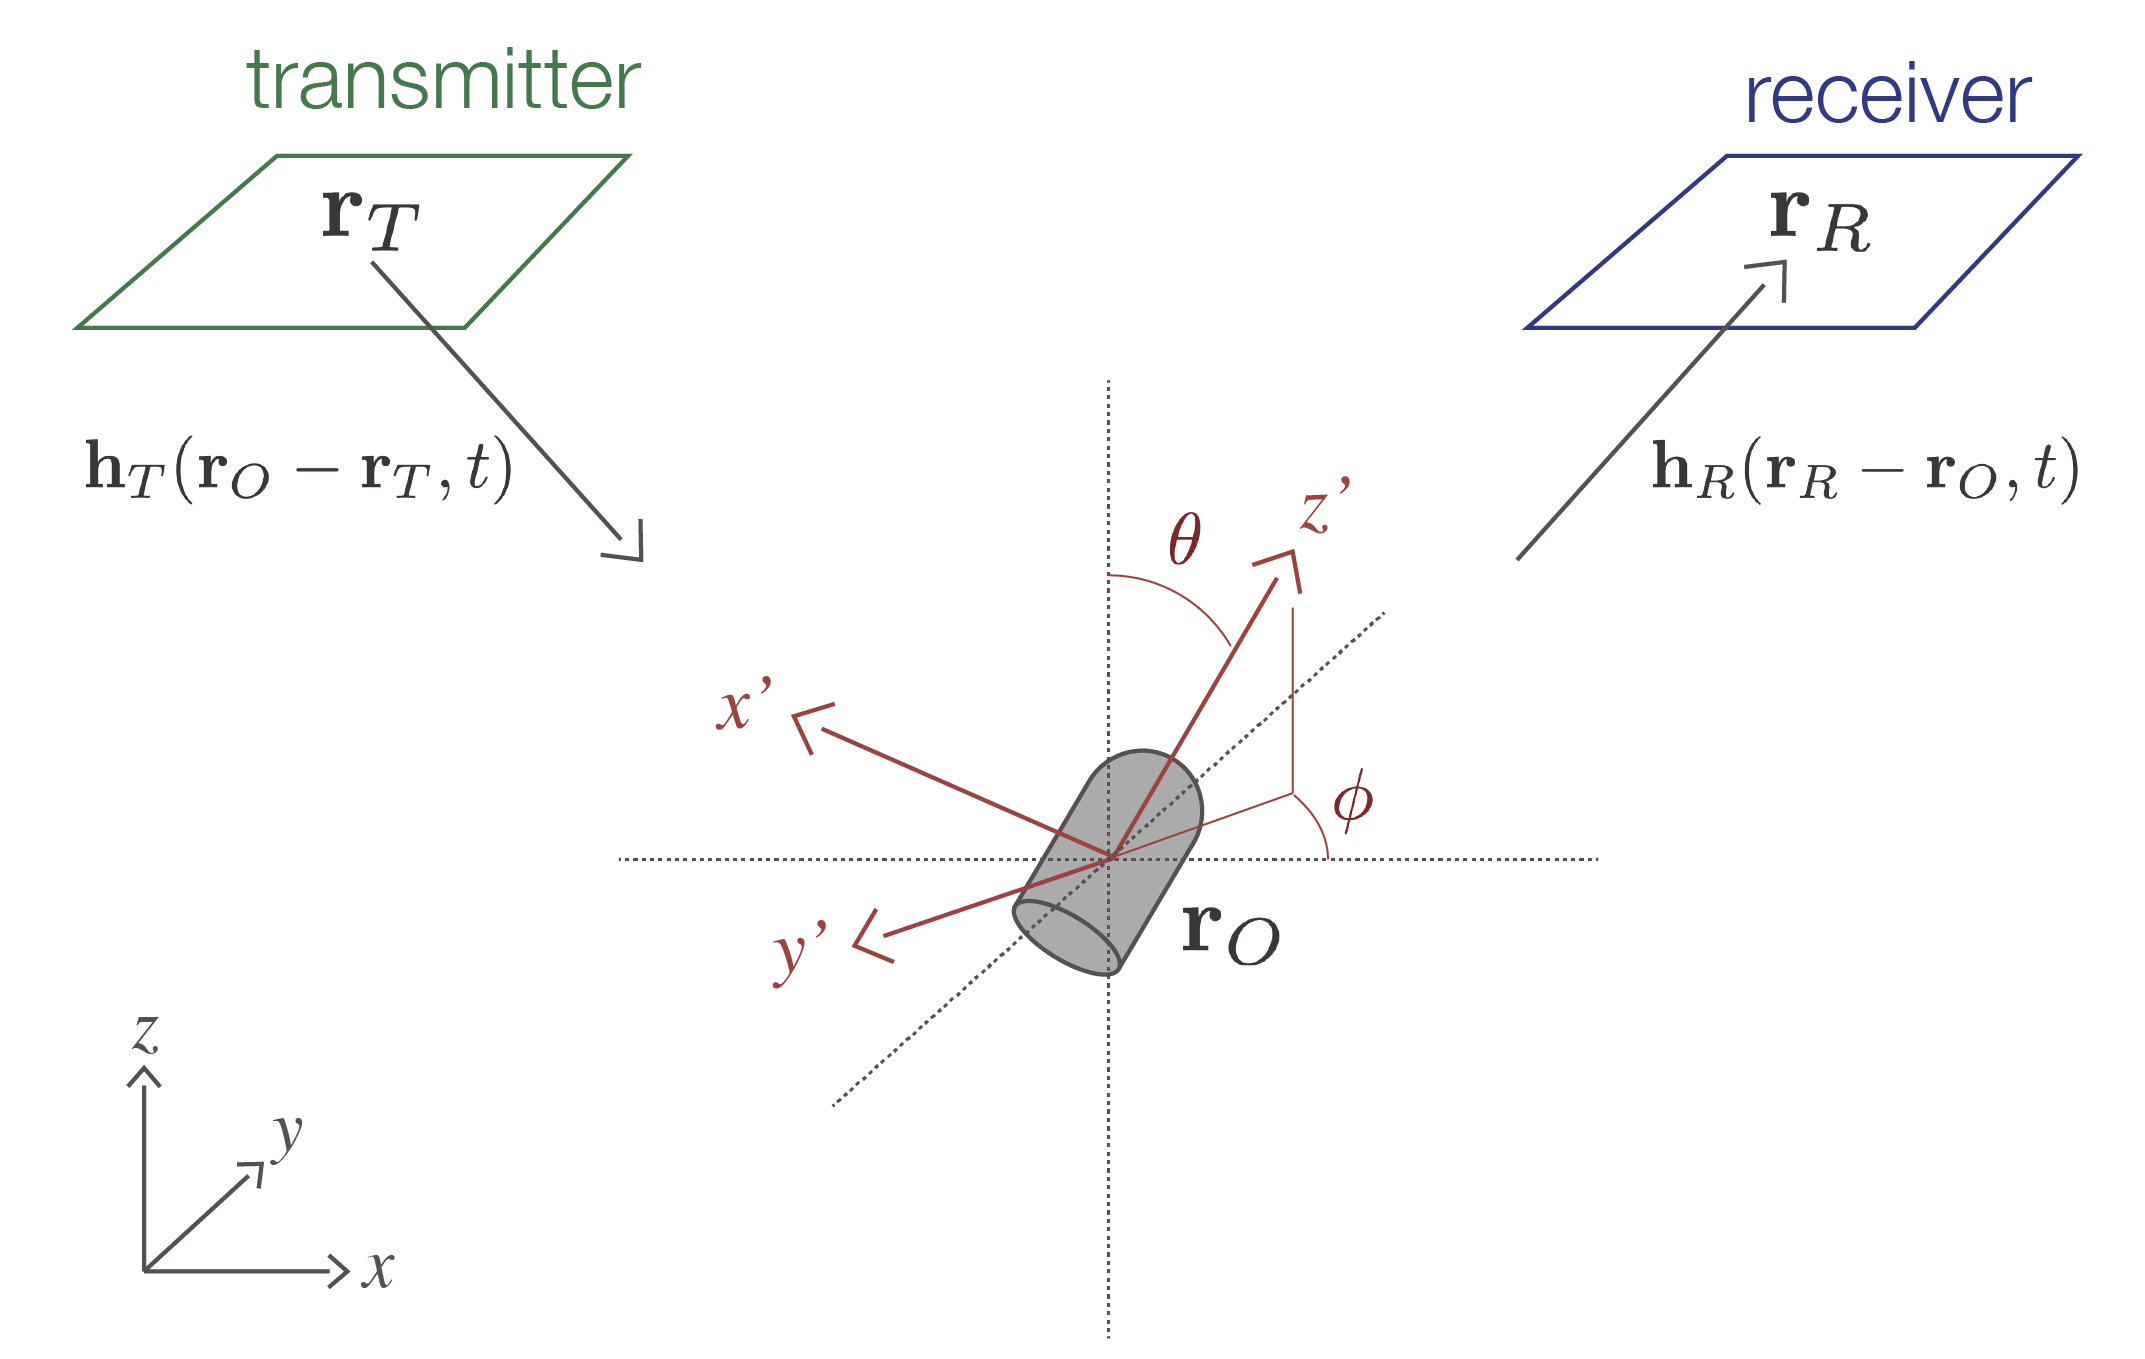
\includegraphics[width=0.85\columnwidth]{figures/uxo-coordinates-01-01.png}
    \end{center}
    % \vspace{-0.5cm}
\caption{
    Electromagnetic experiment to detect a UXO.
    The transmitter produces a primary magnetic field which excites
    currents in a conductive UXO producing a secondary magnetic field
    which is measured at the receiver.
}
\label{fig:uxo-coordinates}
% \vspace{-0.1cm}
\end{figure}

To simulate the electromagnetic response of an unexploded ordnance object, we use an approximate forward model, namely that due to the response of a transient magnetic dipole
\vspace{-0.1cm}
\begin{equation}
    \frac{\partial \mathbf{b}_R}{\partial t}(\mathbf{r}, t) =
    \frac{1}{r^3}\left(3\mathbf{\hat{r}} (\mathbf{\hat{r}} \cdot \mathbf{m}(t) - \mathbf{m(t)}\right)
    \label{eq:uxo-data}
    \vspace{-0.05cm}
\end{equation}

where $\mathbf{r} = r\mathbf{\hat{r}} = \mathbf{r}_R - \mathbf{r}_O$ is the separation between the receiver and the ordnance object \citep{Bell2001, Pasion2001, Zhang2003}. The moment, $\mathbf{m}(t)$, is given by
\vspace{-0.1cm}
\begin{equation}
    \mathbf{m}(t) = \mathbf{P}(t) \cdot \mathbf{h}_T(\mathbf{r}_O - \mathbf{r}_T, t)
    \label{eq:uxo-m}
    \vspace{-0.05cm}
\end{equation}

\cite{Bell2001}. It depends upon the strength of the primary magnetic field at the location of the ordnance object as well as the properties of the object, which are captured in the polarizability tensor
\vspace{-0.1cm}
\begin{equation}
    \mathbf{P}(t) = \mathbf{E}(\phi, \theta, \psi) \cdot \mathbf{L}(t) \cdot \mathbf{E}^\top(\phi, \theta, \psi)
    \label{eq:uxo-P}
    \vspace{-0.05cm}
\end{equation}

The matrix $\mathbf{E}$ is an orthogonal matrix which rotates the coordinate system from the geographic coordinates ($x, y, z$ in Figure \ref{fig:uxo-coordinates}) to the local, body-centered coordinate system of the ordnance object ($x', y', z'$ in Figure \ref{fig:uxo-coordinates}). The polarization matrix $\mathbf{L}(t)$ is a diagonal matrix whose entries are the principal polarizabilities of the ordnance object (in the $x', y', z'$ coordinates):
% \vspace{-0.1cm}
\begin{equation}
    \mathbf{L}(t) = \left(
    \begin{array}{ccc}
    L_1(t) && \\
    & L_2(t) &\\
    && L_3(t)
    \end{array}
    \right)
    \label{eq:uxo-L}
    % \vspace{-0.05cm}
\end{equation}

These polarizabilities depend upon the physical properties of the ordnance object as well as its geometry. For forward modelling, we use the BTInvert Python code, provided by Black Tusk Geophysics.

% \vspace{-0.45cm}
\section{Survey and data}
% \vspace{-0.25cm}

We consider an UltraTEM towed array, with the geometry shown in figure \ref{fig:ultratem} \citep{Billings2018}. The system consists of 5 transmitters and 11 receivers which each measure 3 components of $\partial \mathbf{b}/\partial t$ at 27 time channels between 0.15 ms and 2.5 ms. A sounding collected at a single location of the towed array then consists of 165 time-series EM data ($5 \times 11 \times 3$).
\begin{figure}[htb]
\vspace{-0.1cm}
    \begin{center}
    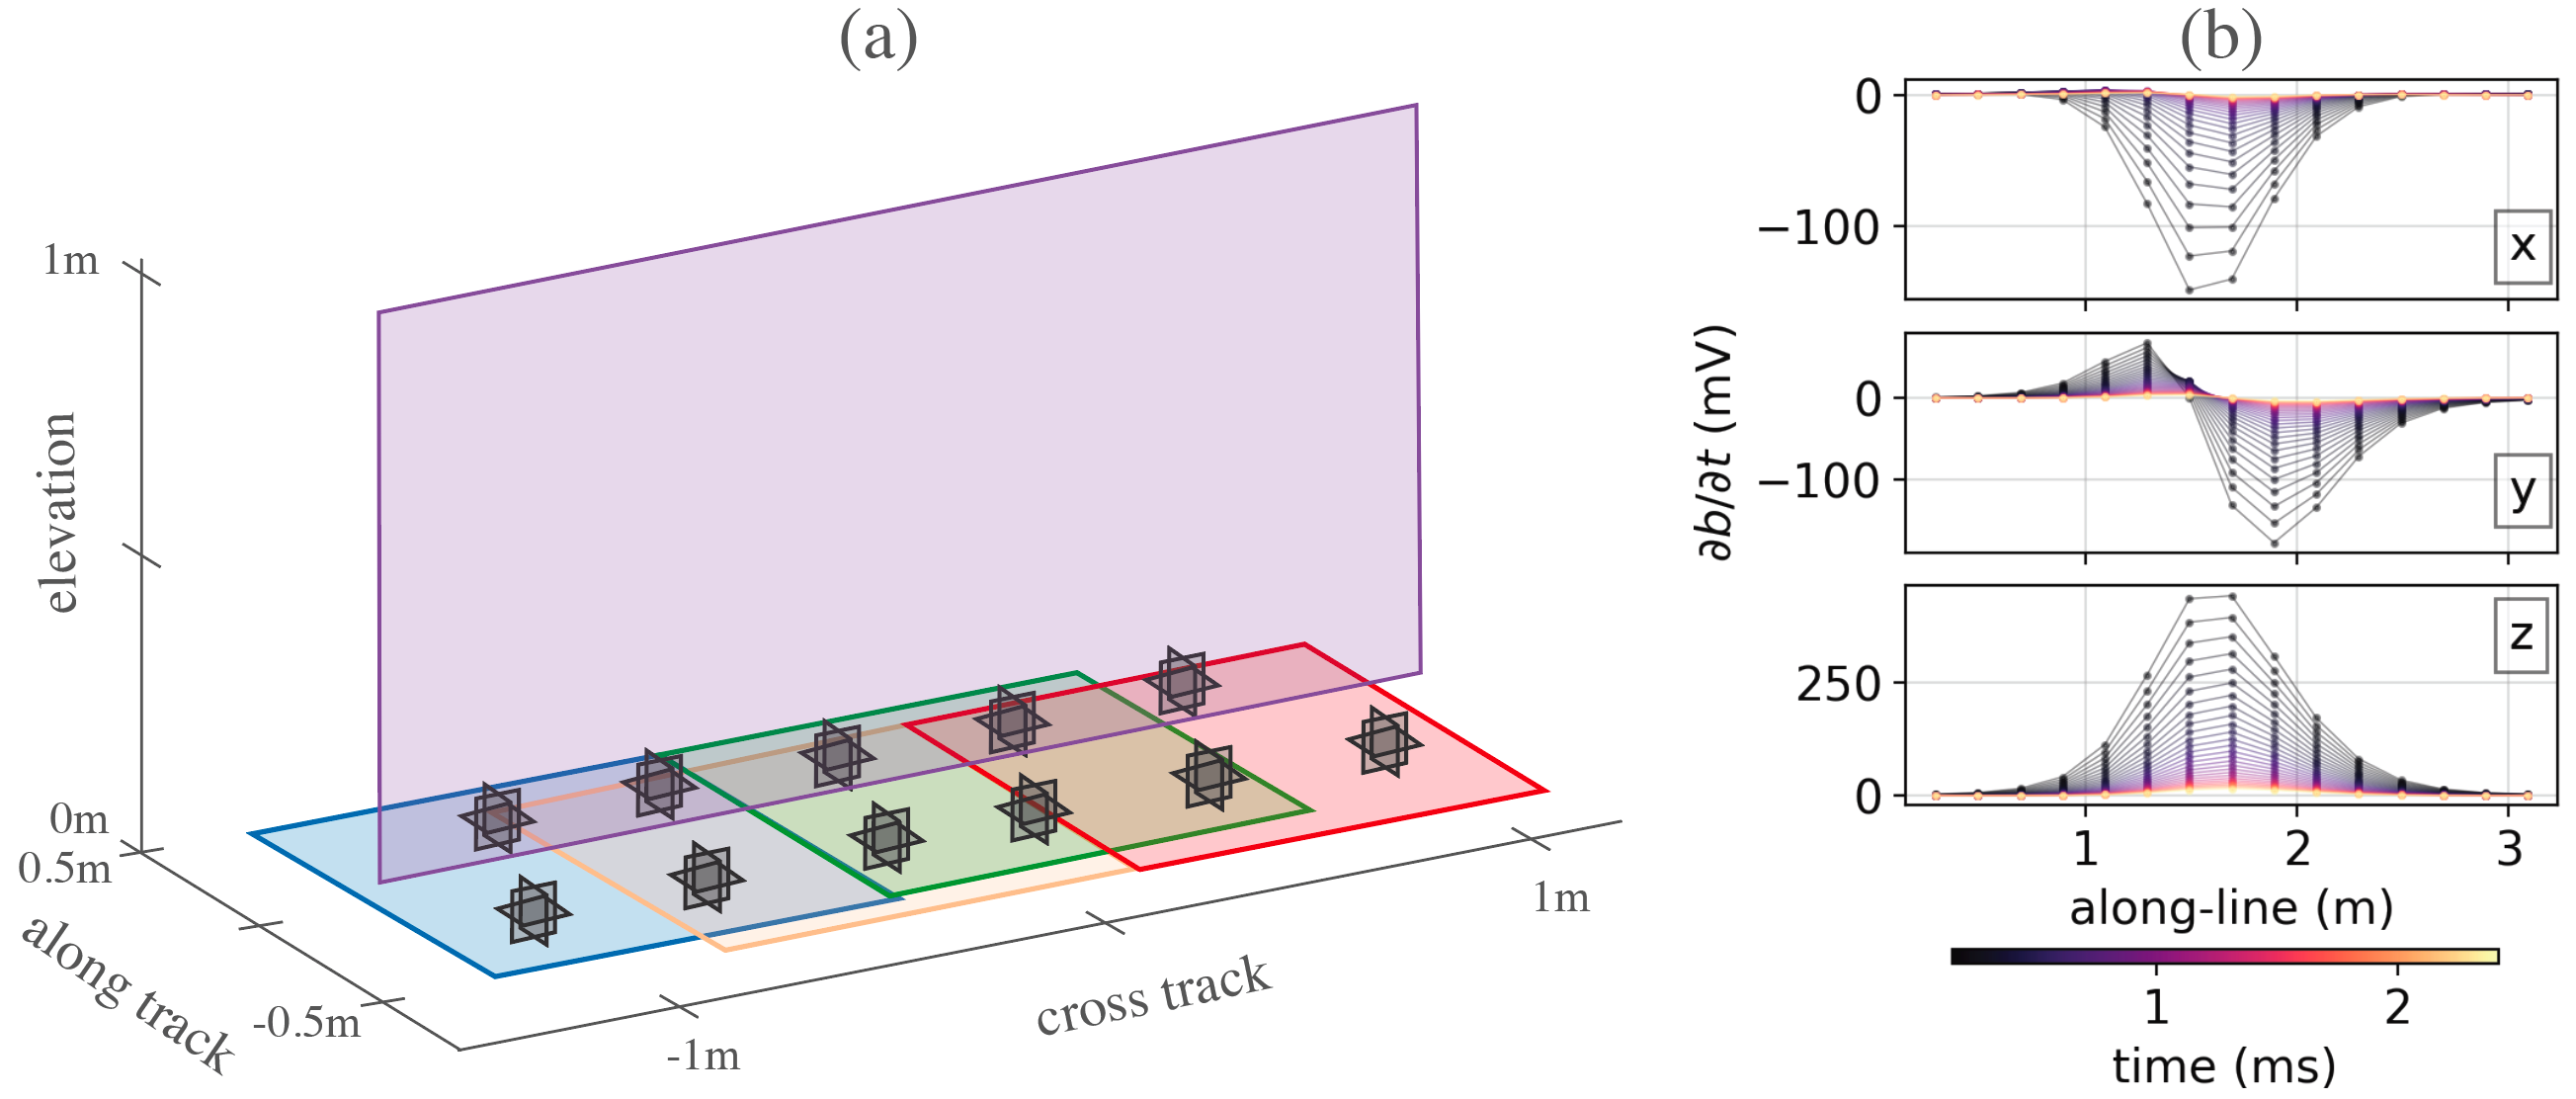
\includegraphics[width=\columnwidth]{figures/ultratem-04.png}
    \end{center}
    \vspace{-0.5cm}
\caption{
    (a) Geometry of the UltraTEM system. Colors indicate transmitters
    and the grey cubes are the three-component $\partial \mathbf{b}/\partial t$ receivers.
    (b) A sample of simulated data (one transmitter and one 3-component receiver) over a Medium ISO. The color of the lines indicates the time-channel.
}
\label{fig:ultratem}
\vspace{-0.1cm}
\end{figure}


A typical approach for working with these data would be to identify regions with anomalous signal, select a subset of data containing the anomaly, and then perform parametric inversions to estimate the location, orientation, and principal polarizabilities of an object. These polarizabilities are used in the classification step where they are matched with a library of known ordnance polarizabilities.


% \vspace{-0.45cm}
\section{Machine learning approach}
% \vspace{-0.25cm}

Rather than going through an inversion process and then classifying objects, our aim is to build a neural network that, given UltraTEM data, classifies the signal as being associated with an ordnance type, clutter, or background.

Convolutional Neural Networks (CNNs) are widely used in applications for images, audio, and video data (e.g. \cite{Krizhevsky2012, LeCun1995, LeCun2010}). Convolutional filters exploit spatial and temporal relationships to learn from the data. CNNs are increasingly being adopted for working with geophysical data. For example they have been applied for seismic horizon tracking \citep{Peters2020} and mineral prospectivity mapping \citep{Granek2016}, among others.

In an image classification problem with color images, the input data would typically include 3 channels of input (red, green and blue), with each channel having an associated $nx \times ny$ image. Analogously, for the UltraTEM data, we have 165 input channels (one for each transmitter-receiver pair), and the size of the ``image'' is the number of along-line data points by number of time-channels (27). Figure \ref{fig:ultratem}(b), shows a sample of 3 of the 165 TDEM profiles over a Medium ISO; these are the data that are input to the network. In the following work, we work with 15 along-line data points, which corresponds to a $\sim$ 3m window. The spacing between measurement points is typical of UltraTEM field data.

The neural network we use consists of 2 convolution layers, followed by a dense layer for classification (also referred to as a fully connected layer). Each of the convolutional layers uses $3 \times 3$ convolutional kernels, batch normalization, a ReLU activation and a max pooling operation. There are 165 input channels, the first convolutional layer outputs 33 channels and the second layer outputs 11. In total, the network has $\sim$75,000 trainable parameters. We denote a forward pass of the network as
\vspace{-0.1cm}
\begin{equation}
    \mathbf{s} = \mathcal{F}_\mathbf{w}(\mathbf{x})
    \label{eq:forward-pass}
    \vspace{-0.05cm}
\end{equation}


where $\mathbf{x}$ is a tensor containing the input features, $\mathbf{w}$ are the trainable weights, and $\mathbf{s}$ are the outputs of the network which has $k$ entries where $k$ is the number of classes. The probability that the feature-set $\mathbf{x}$ is associated with class $j$ is computed via the softmax function (cf. \cite{Hastie2009})
\vspace{-0.1cm}
\begin{equation}
    p(j|\mathbf{s}) = \frac{e^{s_j}}{\sum_{k} e^{s_k}}
    \label{eq:softmax}
    \vspace{-0.05cm}
\end{equation}

The predicted class is then simply the entry with the largest probability
\vspace{-0.1cm}
\begin{equation}
    y_{\rm pred} = \underset{j}{\rm arg\,max} ~~ p(j|\mathbf{s})
    \label{eq:prediction}
    \vspace{-0.05cm}
\end{equation}

The training problem is an optimization problem in the network weights. The loss function we adopt is the cross entropy loss, which is a standard choice for classification problems, giving,
\vspace{-0.1cm}
\begin{equation}
    \min_{\mathbf{w}} \phi = - \sum_k q_k\log(p_k)
    \label{eq:training-problem}
    \vspace{-0.05cm}
\end{equation}

as the statement of the training problem. The label is encoded in $q_k \in {0, 1}$ which takes the value 0 for all entries except the one corresponding to the true class label (referred to as one-hot encoding). Our implementation uses Pytorch \citep{Paszke2019}, and can be accessed at https://github.com/simpeg-research/heagy-et-al-2020-uxo-seg.

To construct the input features $\mathbf{x}$, we perform two normalization steps on the data, which are illustrated in Figure \ref{fig:data-normalizations}. In the first, we scale the data as a function of time-channel and multiply the data at each time by its time-channel (Figure \ref{fig:data-normalizations}b). The purpose of this step is to amplify the influence of late-time channels in the network while still preserving characteristics of the decay, which are indicative of the principal polarizabilities. In the second step, we scale all 165 inputs by the maximum amplitude across all data so that all inputs are in the range $[-1, 1]$ (Figure \ref{fig:data-normalizations}c) . The aim of this step is to force the network to learn spatial and temporal relationships within the data rather than simply the mean amplitude of signal associated with a given ordnance object, which is influenced both by the ordnance type and by the depth of burial.
\begin{figure}[htb]
    \vspace{-0.1cm}
    \begin{center}
    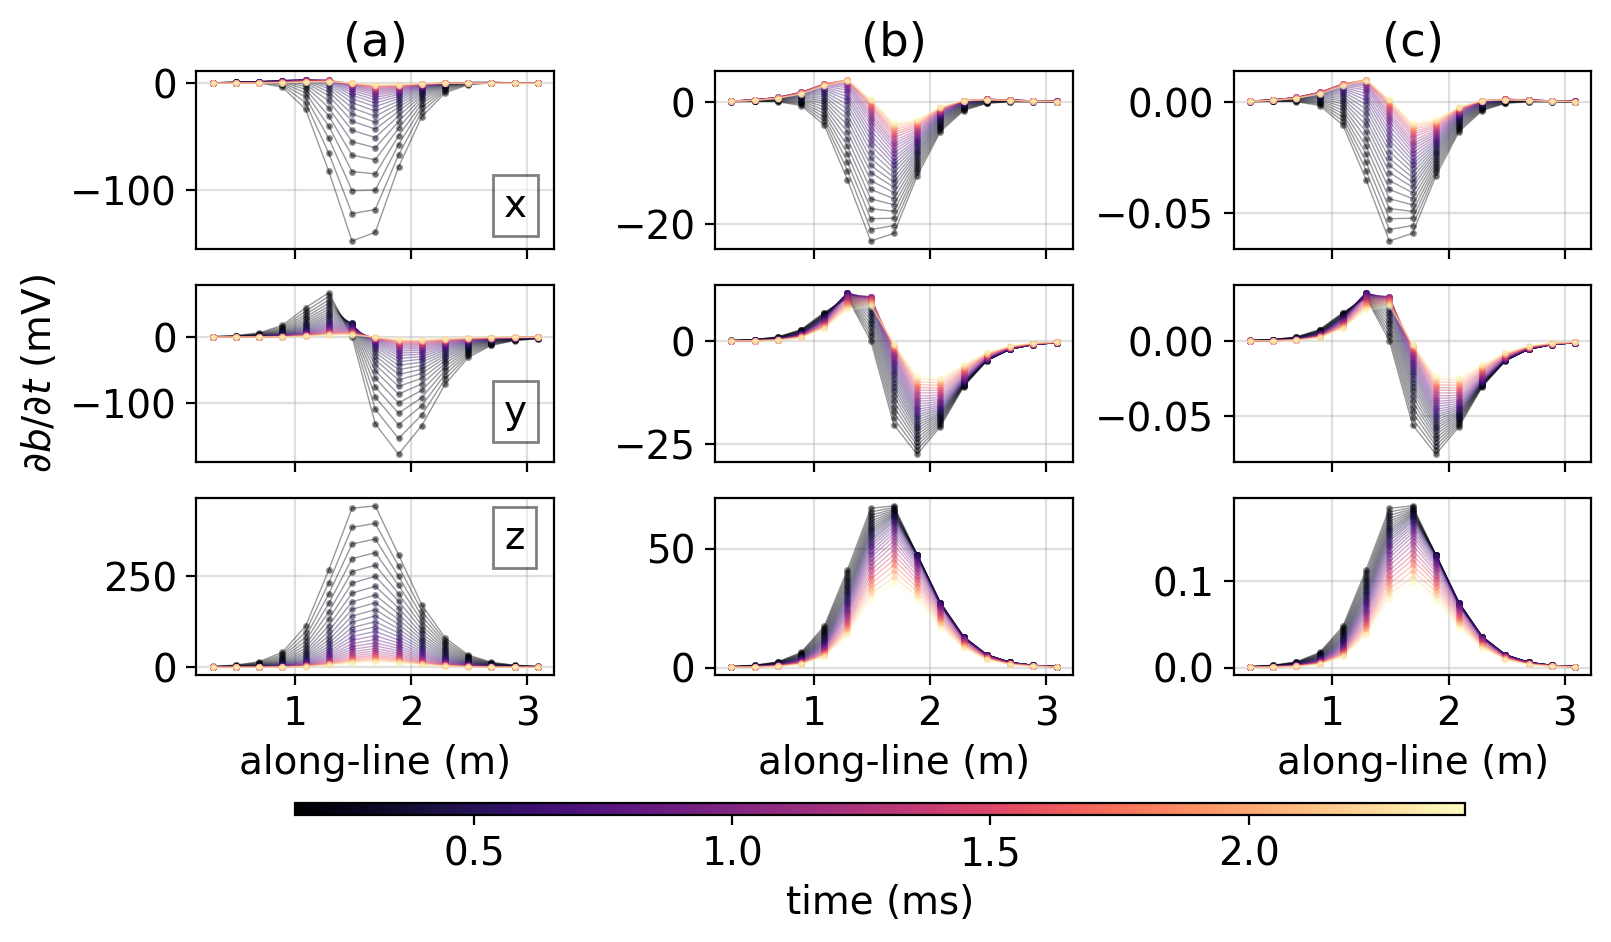
\includegraphics[width=\columnwidth]{figures/data_normalizations.png}
    \end{center}
    \vspace{-0.5cm}
\caption{
    Subset of (a) simulated data,
    (b) data that have been multiplied by $t$, the time-channel (step 1 in the normalizations),
    (c) data from (b) which have been normalized by the maximum amplitude across all 165 inputs.
}
\label{fig:data-normalizations}
\vspace{-0.1cm}
\end{figure}



% \vspace{-0.25cm}
\subsection{Training}
% \vspace{-0.4cm}

We consider 5 classes: background, Small ISO, Medium ISO, Large ISO, and clutter. For each realization we randomly assign the class, noise level, and location and orientation of the target object. The range of parameters is shown in table \ref{tab:parameter-ranges}. The training set we generate consists of 8192 simulations and the test and validation sets each consist of 1024 realizations. For our noise model, we generate gaussian random noise of the form
% \vspace{-0.1cm}
\begin{equation}
    \varepsilon = a \frac{1}{t} \mathcal{N}(0, 1)
    \label{eq:noise}
    % \vspace{-0.05cm}
\end{equation}

where $a$ is the amplitude / variance (in the range specified in Table \ref{tab:parameter-ranges}), $t$ is time (ms) and $\mathcal{N}(0, 1)$ is the standard normal distribution. The functional form of the noise model mimics the $\sim 1/t$ decay expected at intermediate times over a conductive, permeable target \citep{Pasion1999} and is consistent with the noise observed at the test plot.
\begin{table}
    \centering
    \begin{tabular}[htb]{|l|r|}
    \hline
    class & [0, 4] \\ \hline
    x-location (m) & [-1.75, 1.75] \\ \hline
    y-location (m) & [-0.5, 3.5] \\ \hline
    depth (m) & [0, 0.5] \\ \hline
    yaw & [0, 2$\pi$] \\ \hline
    pitch & [0, 2$\pi$] \\ \hline
    % roll & [0, 2$\pi$] \\ \hline
    mean noise amplitude (log sampled) & [$10^{-5}, 10^{-2}$] \\ \hline
    \end{tabular}
    \caption{Range of variable assigned in the training, test, and validation sets.}
    \label{tab:parameter-ranges}
    % \vspace{-0.5cm}
\end{table}

Polarizabilities for each ordnance type are specified by the Department of Defence database \citep{Murray2016}. To simulate clutter, we include both: (a) ordnance objects that are not expected at a given site, here we include the polarizabilities for a 20mm munition, and (b) spherical objects, which have $L_1 = L_2 = L_3$; for the following work, we use the polarizabilities associated with a Small ISO. How to design a ``clutter'' class that includes sufficiently diverse signals that are not associated with targets of interest is an avenue for future development.

We train the network for 10 epochs using stochastic gradient descent and mini-batches of size 32. The training, test, and validation accuracy are 98.7\%, 97.6\%, and 98.2\%, respectively.

To demonstrate the use of the trained classifier for interpreting signal, we consider a single profile of data collected over 3 objects, a Small ISO $(5m, -0.4m)$, a clutter item $(17m, -0.2m)$, and a Medium ISO $(26m, -0.7m)$. The along-line location of each item is indicated by the squares in Figure \ref{fig:profile-line}a (the vertical location of the squares has no meaning). All items are centered in the cross-line direction ($x=0$). To interpret the signal, we consider a moving 3m window and perform a classification for each window of data. This can be thought of as a coarse-scale segmentation problem in machine learning. The classifications are denoted by the circles in Figure \ref{fig:profile-line}a; each circle is the classification of data in a 3m window centered at the location of the dot. To simplify the image, we do not plot classifications of ``background'' in Figure \ref{fig:profile-line}a. Figure \ref{fig:profile-line}b shows the associated class probabilities, computed using equation \ref{eq:softmax}.

Near the along-line center of each target, our classifications are correct and the associated probabilities near 1. Of note is that the training set only included simulations of ordnance objects up to 0.5m depth; the Medium ISO in this example is deeper (0.7m) and the classifications near that object are correct. There are misclassifications and lower probabilities near the edge of the anomalous signals. Our training set only contained some simulations where the item of interest was outside the along-line window of signal we are considering, but only to a maximum of $\pm 0.5m$. The misclassifications are in regions where there is still coherent signal, but the network has not seen training data with objects that are further than 0.5m from the window of interest. How best to treat these ``edge effects'' requires further investigation. We could expand the variability of the training set to include items further away; this would then increase the footprint of the classification. Another alternative is to include simulations of distant objects in the background-class, or perhaps we will require some combination of these approaches.

\begin{figure}[htb]
    \vspace{-0.1cm}
    \begin{center}
    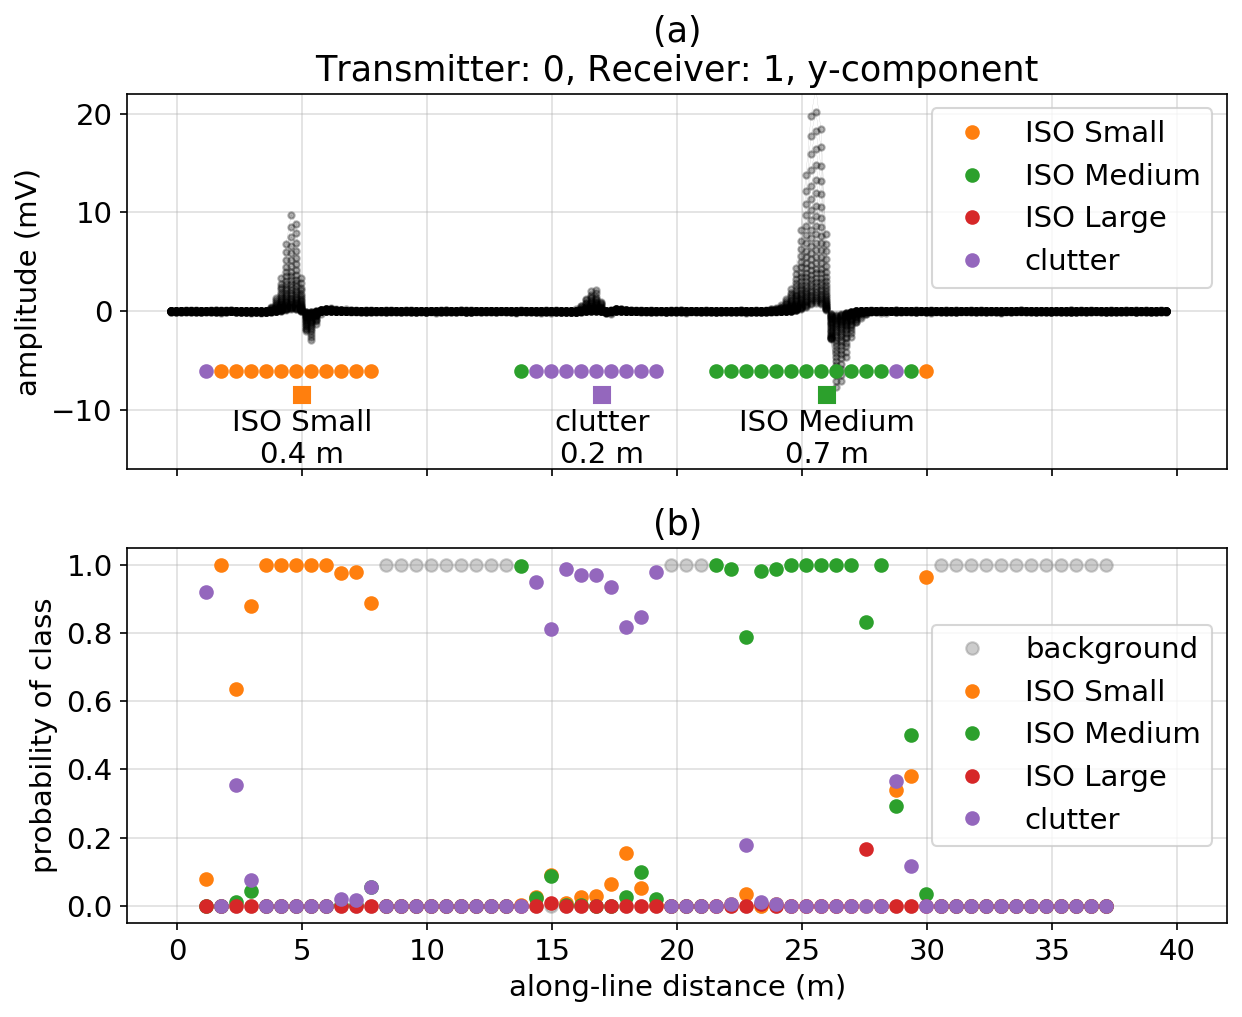
\includegraphics[width=\columnwidth]{figures/profile-line.png}
    \end{center}
    \vspace{-0.5cm}
\caption{
    (a) Simulated UltraTEM data collected along a profile line (black) with 3 items whose along-line location is indicated by the squares.
    The number indicated beneath each item indicates its depth.
    The colored circles denote the classification obtained from the trained neural network for signal within a 3m window that is centered at the along-line location of the circle.
    (b) Probabilities associated with each class.
}
\label{fig:profile-line}
\vspace{-0.1cm}
\end{figure}




% \vspace{-0.45cm}
\section{Synthetic example}
% \vspace{-0.25cm}

We now consider how this approach could be used to produce maps indicating the probability of a given ordnance item at a field site. We construct a synthetic example based on the data collected at a test plot in Australia. Figure \ref{fig:synthetic-test-plot} shows the survey lines (grey) and the location and depth of ordnance items and clutter. These locations and depths were drawn for a subset of the items seeded at the test plot.
\begin{figure}[htb]
% \vspace{-0.1cm}
    \begin{center}
    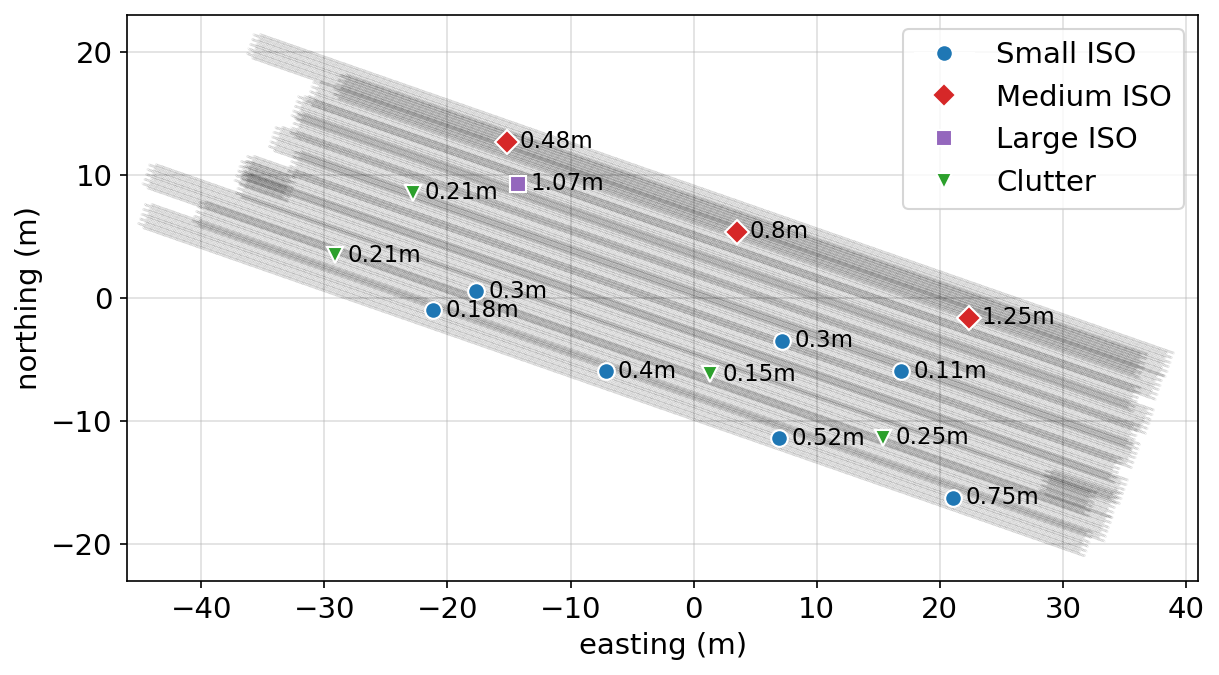
\includegraphics[width=\columnwidth]{figures/synthetic-test-plot.png}
    \end{center}
    % \vspace{-0.5cm}
\caption{
    Survey geometry based on the data collected at a test plot in Australia.
    Ordnance locations are selected from a subset of those seeded at the test plot.
    The values to the right of the markers indicate the depth of each object.
}
\label{fig:synthetic-test-plot}
% \vspace{-0.1cm}
\end{figure}

As was done in the previous section, we use a sliding 3m window and use the trained network to provide probabilities associated with each of the classes. These probabilities are gridded using the block reduce and spline operations included in \textt{verde}  \citep{Uieda2018}. A map of the probabilities for each item are shown in Figure \ref{fig:synthetic-field-probs}. Overall, there is good agreement between where significant probabilities are assigned and the true spatial location of each target object. In Figure \ref{fig:synthetic-field-probs}b, there is a false-positive near (-15m, 5m) easting. We attribute this to ``edge effects'', as we observed in the previous section, due to the Large ISO. Similarly, we see halo-effects in Figure \ref{fig:synthetic-field-probs}d where moderate probabilities are assigned to the clutter class in the vicinity of ordnance objects.
\begin{figure}[htb]
    % \vspace{-0.1cm}
    \begin{center}
    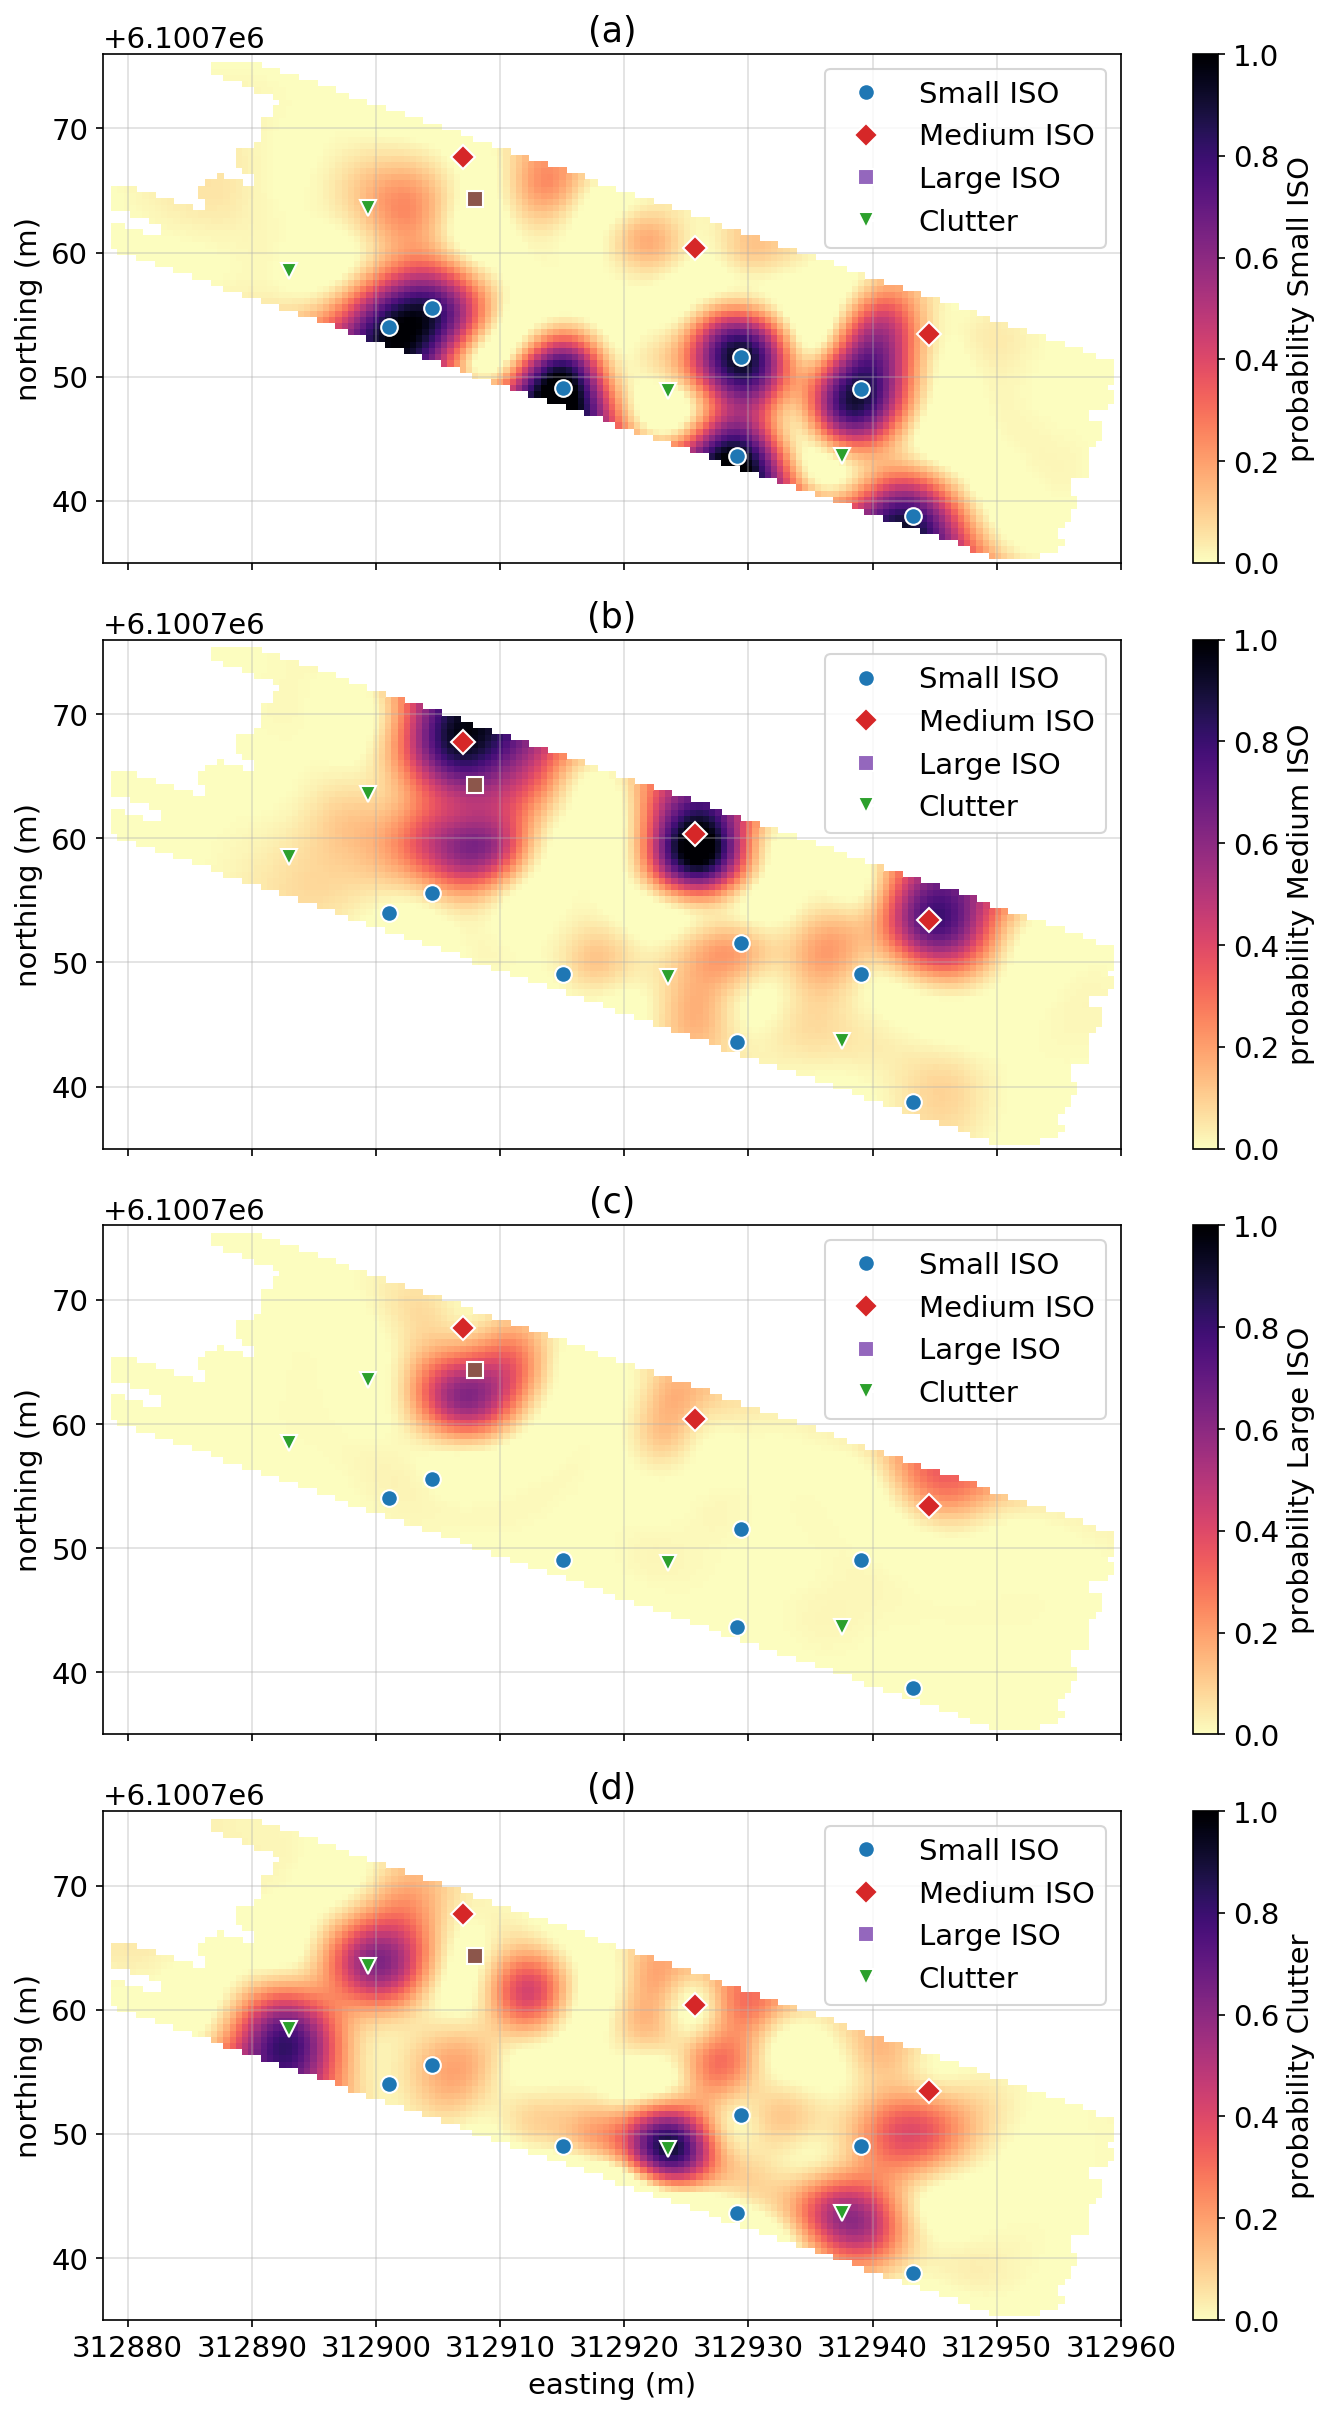
\includegraphics[width=\columnwidth]{figures/synthetic-field-probs.png}
    \end{center}
    % \vspace{-0.5cm}
\caption{
    Maps of the probability of each target class: (a) Small ISO, (b) Medium ISO, (c) Large ISO, (d) Clutter.
}
\label{fig:synthetic-field-probs}
% \vspace{-0.1cm}
\end{figure}


% \vspace{-0.45cm}
\section{Discussion and conclusions}
% \vspace{-0.25cm}

The problem of classifying unexploded ordnance from electromagnetic data has several characteristics that make it a good candidate for the use of CNNs: we are able to construct synthetic labeled training sets from a library of known ordnance objects, there are labeled field data sets, and the data acquired from a given EM system (e.g. the UltraTEM) have a spatio-temporal structure that is well suited for the classification strengths of CNNs. The synthetic results we have shown demonstrate the potential for neural networks to be a useful interpretation tool to augment inversion-based approaches. The method we present could be used to prioritize areas where a cued sensor may be deployed to collect longer off-time data, or to provide an independent interpretation to complement an inversion result.

This work is in early stages, and there are open questions with respect to constructing robust noise and clutter models, handling multi-object scenarios where two or more ordnance items are in close proximity, as well as addressing challenging geologic scenarios such as settings with magnetic soils which complicate the EM response. Additionally, we plan to further investigate strategies for designing the network architecture, input features, and the loss function (e.g. incorporating the asymmetry between the consequences of false positives and false negatives). The CNN architecture we presented is specific to the geometry of the UltraTEM system, however, we anticipate that this approach could be readily adapted to other multi-component EM systems.

% \vspace{-0.45cm}
\section{Acknowledgements}
% \vspace{-0.25cm}

The authors are grateful to David Sinex, Len Pasion, Lin-Ping Song, and Nicolas Lhomme for constructive conversations on the setup of this problem, for providing background information in the UltraTEM system, as well as support on the use of BTInvert. We are also grateful to Josh Bloom for conversations on neural network architectures.
Thanks to Black Tusk Geophysics for providing data from the test plot which motivated the synthetic example used in this paper, as well as for providing access to BTInvert.

\onecolumn


\bibliographystyle{seg}  % style file is seg.bst
\bibliography{uxo}

\end{document}
